% !TeX program = xelatex
% =============================================================================
%  DỰ ÁN TỐT NGHIỆP — BÁO CÁO CHUYÊN ĐỀ
%  Đề tài: Phân tích Hiệu suất và Dự báo Sản lượng Hệ thống Điện Mặt Trời
%  Nhóm: The Outliers
%  Trường: Cao đẳng FPT Polytechnic — Chuyên ngành Xử lý Dữ liệu
% =============================================================================

\documentclass[12pt, a4paper]{report}

% ======================== PACKAGES CƠ BẢN & FONT ============================
\usepackage{geometry}
\geometry{a4paper, top=2.5cm, bottom=2.5cm, left=3cm, right=2cm, headheight=33pt, footskip=1.1cm}

% --- FONT CHO XELATEX (HỖ TRỢ TIẾNG VIỆT 100% - FORMAL, TỐI GIẢN, HIỆN ĐẠI) ---
\usepackage{fontspec}
\setmainfont{Times New Roman}
\setmonofont{Consolas}

% ======================== MÀU SẮC & CODE LISTINGS ===========================
\usepackage{xcolor}
\usepackage{listings}
% Định nghĩa bảng màu Tableau trích xuất từ main_fixed_01.twb & tableau_theme.json
\definecolor{tblNavy}{HTML}{4E79A7}
\definecolor{tblOrange}{HTML}{F28E2B}
\definecolor{tblGreen}{HTML}{59A14F}
\definecolor{tblRed}{HTML}{E15759}
\definecolor{tblTeal}{HTML}{76B7B2}
\definecolor{tblYellow}{HTML}{EDC948}
\definecolor{tblPurple}{HTML}{B07AA1}
\definecolor{tblGray}{HTML}{79706E}
\definecolor{tblSeqWarm}{HTML}{F28E2B}

% Định nghĩa màu sắc cho Code Block
\definecolor{mutedgreen}{rgb}{0.2,0.5,0.3} 
\definecolor{mutedblue}{rgb}{0.15,0.35,0.6} 
\definecolor{mutedgray}{rgb}{0.45,0.45,0.45} 
\definecolor{mutedpurple}{rgb}{0.45,0.2,0.55} 
\definecolor{softbackground}{rgb}{0.98,0.98,0.98} 
\definecolor{bordergray}{rgb}{0.85,0.85,0.85} 
\definecolor{fptorange}{RGB}{245,130,32}

\lstdefinestyle{pythonstyle}{
    backgroundcolor   = \color{softbackground},
    commentstyle      = \color{mutedgreen}\itshape,
    keywordstyle      = \color{mutedblue}\bfseries,
    numberstyle       = \tiny\color{mutedgray},
    stringstyle       = \color{mutedpurple},
    basicstyle        = \ttfamily\footnotesize\color{black},
    breakatwhitespace = false,
    breaklines        = true,
    columns           = fullflexible,
    captionpos        = t, 
    keepspaces        = true,
    numbers           = left,
    numbersep         = 5pt,
    showspaces        = false,
    showstringspaces  = false,
    showtabs          = false,
    tabsize           = 4,
    frame             = single,
    rulecolor         = \color{bordergray}
}
\lstset{style=pythonstyle}

% Ngăn chặn tự động gạch nối từ (hyphenation) cuối dòng
\hyphenpenalty=10000
\exhyphenpenalty=10000
\tolerance=10000
\emergencystretch=3em

% ======================== TRANG TRÍ & ĐỊNH DẠNG =============================
\usepackage{fancyhdr}
\usepackage{lastpage}
\usepackage{amsmath, amssymb}
\usepackage{enumitem}
\usepackage{array}
\newcolumntype{L}[1]{>{\raggedright\arraybackslash}p{#1}}
\newcolumntype{C}[1]{>{\centering\arraybackslash}p{#1}}
\newcolumntype{R}[1]{>{\raggedleft\arraybackslash}p{#1}}
\usepackage{booktabs}
\usepackage{tabularx}
\usepackage{longtable}
\usepackage{multirow}
\usepackage{graphicx}
\graphicspath{{images/}{figures/}{./}}
\usepackage{float}
\usepackage{caption}
\usepackage{subcaption}
\usepackage{tikz}
\usepackage[titles]{tocloft}

% VIỆT HÓA TOÀN BỘ CÁC TIÊU ĐỀ HỆ THỐNG
\renewcommand{\figurename}{Hình}
\renewcommand{\tablename}{Bảng}
\renewcommand{\contentsname}{Mục Lục}
\renewcommand{\listfigurename}{Danh Mục Hình Vẽ}
\renewcommand{\listtablename}{Danh Mục Bảng Biểu}
\providecommand{\tep}[1]{\texttt{#1}}

\usepackage{indentfirst}
\setlength{\parindent}{1cm}
\setlength{\parskip}{6pt}

\usepackage{setspace}
\onehalfspacing
\setlength{\headheight}{33pt}

% Hyperlinks & Bookmarks
\usepackage{hyperref}
\hypersetup{
    colorlinks  = true,
    linkcolor   = black,
    citecolor   = blue,
    filecolor   = magenta,
    urlcolor    = blue,
    pdftitle    = {Dự án Tốt nghiệp - Phân tích Hiệu suất và Dự báo Sản lượng Hệ thống Điện Mặt Trời},
    pdfauthor   = {The Outliers - FPT Polytechnic},
    bookmarksnumbered = true,
}

% --- CẤU HÌNH TIÊU ĐỀ CHƯƠNG ---
\usepackage{titlesec}
\titleformat*{\section}{\fontsize{13pt}{15.6pt}\bfseries}
\titleformat*{\subsection}{\fontsize{13pt}{15.6pt}\bfseries}
\titleformat*{\subsubsection}{\fontsize{13pt}{15.6pt}\bfseries}
\titleformat{\chapter}[display]
  {\normalfont\huge\bfseries}{}{0pt}{\huge}
\titlespacing*{\chapter}{0pt}{-10pt}{20pt} 

% ======================== HEADER / FOOTER ====================================
\fancypagestyle{main}{
    \fancyhf{}
    \fancyhead[L]{
\includegraphics[height=1cm]{figures/logo_fpoly.png}}
    \fancyhead[R]{\small THE OUTLIERS}
    \fancyfoot[L]{\small Dự án Tốt nghiệp — Chuyên ngành Xử lý Dữ liệu}
    \fancyfoot[R]{\small Trang \thepage\ / \pageref{LastPage}}
    \renewcommand{\headrulewidth}{0.4pt}
    \renewcommand{\footrulewidth}{0.4pt}
}

\fancypagestyle{plain}{
    \fancyhf{}
    \fancyfoot[L]{\small Dự án Tốt nghiệp — Chuyên ngành Xử lý Dữ liệu}
    \fancyfoot[R]{\small Trang \thepage\ / \pageref{LastPage}}
    \renewcommand{\headrulewidth}{0pt}
    \renewcommand{\footrulewidth}{0.4pt}
}

\fancypagestyle{front}{
    \fancyhf{}
    \fancyfoot[L]{\small Dự án Tốt nghiệp — Chuyên ngành Xử lý Dữ liệu}
    \fancyfoot[R]{\small Trang \thepage\ / \pageref{LastPage}}
    \renewcommand{\headrulewidth}{0pt}
    \renewcommand{\footrulewidth}{0.4pt}
}


\begin{document}
\pagestyle{front}

\begin{titlepage}
\enlargethispage{1.2cm}

\begin{tikzpicture}[remember picture, overlay]
    \draw[line width=2pt, fptorange]
        ([shift={(1cm,-1cm)}]current page.north west)
        rectangle
        ([shift={(-1cm,1cm)}]current page.south east);
    \draw[line width=0.5pt, fptorange]
        ([shift={(1.15cm,-1.15cm)}]current page.north west)
        rectangle
        ([shift={(-1.15cm,1.15cm)}]current page.south east);
\end{tikzpicture}

\begin{center}
    \textbf{\large TRƯỜNG CAO ĐẲNG FPT POLYTECHNIC}

    \vspace{0.5cm}
    
\includegraphics[width=0.38\textwidth]{figures/logo_fpoly.png}

    \vspace{0.4cm}
    {\Large \textbf{DỰ ÁN TỐT NGHIỆP}} \\[4pt]
    {\large \textbf{CHUYÊN NGÀNH: XỬ LÝ DỮ LIỆU}}

    \vspace{1.6cm}
    
    \begin{spacing}{1.0}
        {\huge \textbf{PHÂN TÍCH HIỆU SUẤT VÀ \\[4pt] DỰ BÁO SẢN LƯỢNG \\[4pt] HỆ THỐNG ĐIỆN MẶT TRỜI}}
    \end{spacing}

    \vspace{1.8cm}
    \normalsize
    \begin{flushleft}
        \hspace{2cm} \textbf{Nhóm thực hiện:} The Outliers \\[5pt]
        \hspace{2cm} \textbf{Sinh viên thực hiện:} \\[3pt]
        \hspace{2cm}
        \begin{tabular*}{7.5cm}{@{} l @{\extracolsep{\fill}} r @{}}
            \hspace{0.5cm} 1. Nguyễn Vũ Nhựt   & PS44442 \\
            \hspace{0.5cm} 2. Nguyễn Văn Sỹ    & PS43671 \\
            \hspace{0.5cm} 3. Lê Công Toàn    & PS44145 \\
            \hspace{0.5cm} 4. Nguyễn Xuân Hùng & PS44527 \\
            \hspace{0.5cm} 5. Ngô Tấn Đạt     & PS44589 \\
        \end{tabular*} \\[5pt]
        \hspace{2cm} \textbf{Giảng viên hướng dẫn:} Văn Công Khanh
    \end{flushleft}
    \vfill
    {\normalsize \textbf{TP. HỒ CHÍ MINH, THÁNG 6 NĂM 2026}}
    \vspace{0.5cm}
\end{center}
\end{titlepage}


\pagenumbering{arabic}
\pagestyle{main}

% ====================================================================
%  CHƯƠNG 3: QUY TRÌNH ETL VÀ MÔ HÌNH HÓA DỮ LIỆU
% ====================================================================
\chapter{Thu thập, Tiền xử lý và Mô hình hóa Kho Dữ liệu}
\label{chap:etl_modeling}

\section{Tổng quan Kiến trúc Pipeline Xử lý Dữ liệu}
\label{sec:pipeline_overview}

Để đảm bảo tính tự động hóa, độ chính xác cao và khả năng tái sử dụng khi có dữ liệu phát sinh mới từ các trạm pin, dự án không xử lý dữ liệu thủ công trên Excel mà thiết kế một quy trình xử lý dữ liệu tự động hoàn chỉnh bằng ngôn ngữ Python. Toàn bộ luồng thực thi từ khâu tải dữ liệu, tiền xử lý, điền khuyết chuỗi thời gian, lọc dữ liệu ngoại lai, nạp vào kho dữ liệu Supabase DWH đến việc xây dựng các siêu thị dữ liệu (Data Marts) được điều phối thông suốt thông qua kiến trúc mô-đun độc lập (Hình~\ref{fig:code_execution_pipeline}).

\begin{figure}[H]
    \centering
    
\includegraphics[width=\textwidth]{figures/code_execution_pipeline.png}
    \caption{Sơ đồ luồng thực thi quy trình xử lý dữ liệu tự động (Code Execution Pipeline).}
    \label{fig:code_execution_pipeline}
\end{figure}

Toàn bộ quy trình được tổ chức thành các mô-đun chức năng độc lập:
\begin{enumerate}[label=\arabic*., leftmargin=*]
    \item \textbf{\texttt{config.py}:} Khởi tạo môi trường, cấu hình thông tin kết nối CSDL Supabase, thiết lập hệ thống ghi vết nhật ký (ghi vết nhật ký hệ thống) và định nghĩa các tham số nghiệp vụ (ngưỡng cắt trần công suất danh định $P_{\text{stc}}$, ngưỡng bức xạ ban đêm $GHI \le 25\,\text{W/m}^2$, đơn giá điện FiT).
    \item \textbf{\texttt{eda.py}:} Quét toàn diện tập dữ liệu thô ($2.731.946$ dòng), kiểm tra dữ liệu thiếu, trùng lặp và phát hiện các điểm đứt gãy thời gian.
    \item \textbf{\texttt{cleaner.py}:} Thực hiện làm sạch dữ liệu, xử lý đứt gãy thời gian bằng Resampling 15 phút, áp dụng 5 rào chắn vật lý và mô hình phân lớp lai GMM--IF để lọc sạch nhiễu cảm biến, gắn 6 mã lý do kỹ thuật và trích xuất đặc trưng nghiệp vụ (trích xuất đặc trưng nghiệp vụ).
    \item \textbf{\texttt{splitter.py}:} Tách bảng phẳng khổng lồ thành mô hình Lược đồ Thiên hà (Galaxy Schema) gồm 2 bảng Fact và 4 bảng Dimension.
    \item \textbf{\texttt{aggregate.py}:} Tạo các bảng tổng hợp (Siêu thị dữ liệu chuyên đề) tính toán trước các chỉ số KPI theo ngày, tháng, trạm phát nhằm tối ưu hóa hiệu năng tải biểu đồ cho Tableau Dashboard.
    \item \textbf{\texttt{main.py}:} Tệp thực thi trung tâm, tự động hóa toàn bộ luồng ETL từ đầu đến cuối chỉ với một dòng lệnh duy nhất.
\end{enumerate}

\section{Đánh giá Chất lượng và Khám phá Dữ liệu (EDA)}
\label{sec:eda_quality}

Trước khi can thiệp vào dữ liệu, hệ thống thực thi module \texttt{eda.py} để kiểm định chất lượng $2.731.946$ bản ghi sản lượng nhằm trả lời câu hỏi cốt lõi: \textit{``Dữ liệu có đáng tin cậy để đưa vào phân tích kinh doanh hay không?''}.

\subsection{Kiểm tra Dữ liệu Thiếu, Trùng lặp và Đứt gãy Chuỗi Thời gian (điểm gián đoạn thời gian)}
Thông qua các thuật toán kiểm định chất lượng dữ liệu bằng Pandas, nhóm đã phát hiện các vấn đề kỹ thuật quan trọng:
\begin{itemize}[noitemsep]
    \item \textbf{Dữ liệu trùng lặp:} Phát hiện 38 cặp bản ghi trùng lặp mã trạm và mốc thời gian, được tự động loại bỏ để giữ lại bản ghi mới nhất (\texttt{keep='last'}).
    \item \textbf{Lỗ hổng Đứt gãy Thời gian (561 điểm gián đoạn thời gian):} Phát hiện 561 điểm nhảy cóc thời gian (chiếm $0{,}0247\%$ tổng dữ liệu) do lỗi đường truyền viễn thông của trạm phát về trung tâm. Đây là phát hiện quan trọng, vì nếu không xử lý liên tục chuỗi thời gian, các phép tính toán trung bình trượt và biến động ngày/đêm sẽ bị sai lệch hoàn toàn.
    \item \textbf{Nhiễu Cảm biến Ban đêm (Dòng rò ban đêm):} Hơn 18.000 bản ghi ghi nhận sản lượng dương ($E > 0$) vào các khung giờ từ 22h đêm đến 4h sáng khi bức xạ triệt tiêu hoàn toàn ($GHI = 0$).
\end{itemize}

\section{Làm sạch và Chuẩn hóa Dữ liệu (Data Cleaning)}
\label{sec:data_cleaning}

\subsection{Chuẩn hóa Cấu trúc Cột và Xử lý Lỗi Logic}
Tệp dữ liệu gốc chứa các tên cột dạng \texttt{PascalCase} và khoảng trắng (như \texttt{SiteKey}, \texttt{SolarGeneration}, \texttt{CampusKey}). Module \texttt{cleaner.py} tự động chuẩn hóa toàn bộ về định dạng chuẩn \texttt{snake\_case} và ép đúng kiểu dữ liệu số thực:

\begin{lstlisting}[language=Python, caption={Đoạn mã Python chuẩn hóa cấu trúc cột sang snake\_case}, label={lst:clean_columns}]
# cleaner.py — Chuan hoa ten cot sang snake_case va loai bo ky tu thua
df.columns = (
    df.columns
    .str.strip()
    .str.lower()
    .str.replace(" ", "_", regex=False)
    .str.replace(".", "_", regex=False)
)
# Ep kieu du lieu thoi gian va so thuc
df["timestamp"] = pd.to_datetime(df["timestamp"])
val_num = pd.to_numeric(df["energy_generated_kwh"], errors="coerce")
    df["energy_generated_kwh"] = val_num.fillna(0.0)
\end{lstlisting}

\subsection{Xử lý Dữ liệu Ngoại lai (Outliers) và Gán Mã Lý do Kỹ thuật}
Thay vì xóa bỏ dữ liệu ngoại lai một cách cơ học (dễ làm mất dấu vết sự cố hỏng hóc thiết bị thực tế), dự án kết hợp 5 quy tắc rào chắn vật lý và mô hình phân lớp lai GMM--IF để nhận diện chính xác $33.280$ dòng dị thường ($1{,}22\%$), đồng thời gán 6 mã lý do kỹ thuật chuẩn hóa (\texttt{gmm\_if\_outlier\_reason}):

\begin{table}[H]
\centering
\small
\renewcommand{\arraystretch}{1.25}
\begin{tabularx}{\textwidth}{@{} l l X @{}}
\toprule
\textbf{Mã Lý do Dị thường} & \textbf{Tỷ lệ (\%)} & \textbf{Ý nghĩa Nghiệp vụ \& Hướng Xử lý} \\
\midrule
\texttt{GMM\_IF\_CONSENSUS} & 0.45\% & Dị thường đa chiều được GMM và IF đồng thuận xác nhận. \\
\texttt{PHYSICAL\_OVER\_CAPACITY} & 0.08\% & Vượt trần công suất danh định ($E > 1{,}25 \cdot P_{\text{stc}} \cdot 0{,}25\text{h}$) do lỗi cảm biến đo. \\
\texttt{PHYSICAL\_HIGH\_ENERGY\_NO\_SUN} & 0.42\% & Phát điện ban đêm ($GHI \le 25\,\text{W/m}^2, E > 0$) $\rightarrow$ Trôi mốc 0 cảm biến CT. \\
\texttt{PHYSICAL\_HIGH\_ENERGY\_LOW\_RAD} & 0.12\% & Bức xạ yếu nhưng sản lượng cao bất thường $\rightarrow$ Xung điện áp lưới. \\
\texttt{PHYSICAL\_LOW\_ENERGY\_STRONG\_SUN} & 0.09\% & Nắng gắt ($GHI \ge 700\,\text{W/m}^2$) mất phát $\rightarrow$ Biến tần ngắt mạch/quá nhiệt. \\
\texttt{PHYSICAL\_DISTRIBUTION\_JUMP} & 0.06\% & Bước nhảy phân bố sản lượng cục bộ đột ngột $\rightarrow$ Lỗi truyền thông. \\
\bottomrule
\end{tabularx}
\caption{Bảng phân loại 6 mã lý do dị thường phục vụ công tác bảo trì O\&M.}
\label{tab:outlier_reasons}
\end{table}

\section{Trích xuất Đặc trưng Nghiệp vụ (trích xuất đặc trưng nghiệp vụ)}
\label{sec:feature_engineering}

Đây là bước tạo ra các chỉ số nghiệp vụ đo lường mới từ dữ liệu thô, cung cấp góc nhìn phân tích đa chiều cho hệ thống BI:

\subsection{Đặc trưng Vận hành và Hiệu suất Kỹ thuật}
Module \texttt{cleaner.py} tự động tính toán các chỉ số vận hành cốt lõi:
\begin{lstlisting}[language=Python, caption={Đoạn mã Python trích xuất các đặc trưng vận hành và tài chính}, label={lst:engineer_features}]
# 1. Tinh san luong ly thuyet theo buc xa thuc te (Theoretical Energy)
rad_factor = df["shortwave_radiation"] / 1000.0
    df["theoretical_energy_kwh"] = df["capacity_kw"] * rad_factor * 0.25

# 2. He so hieu suat quang dien (Performance Ratio - PR)
theo_e = df["theoretical_energy_kwh"].replace(0, np.nan)
    df["pr_pct"] = (df["energy_generated_kwh"] / theo_e) * 100.0
df["pr_pct"] = df["pr_pct"].clip(lower=0.0, upper=120.0)

# 3. Nang suat rieng (Specific Yield - kWh/kWp)
df["specific_yield"] = df["energy_generated_kwh"] / df["capacity_kw"]

# 4. Ton that uoc tinh do nhiet do cao vuot nguong 25 do C (Thermal Loss)
df["temp_loss_kwh"] = np.where(
    df["temperature_2m"] > 25.0,
    df["capacity_kw"] * 0.004 * (df["temperature_2m"] - 25.0) * 0.25,
    0.0
)
\end{lstlisting}

\subsection{Đặc trưng Thời gian Chu kỳ}
Trích xuất các chiều thời gian phục vụ phân tích xu hướng tăng trưởng (YoY), tính mùa vụ và so sánh ngày nghỉ:
\begin{itemize}[noitemsep]
    \item Năm (\texttt{year}), Tháng (\texttt{month}), Quý (\texttt{quarter}), Giờ trong ngày (\texttt{hour}).
    \item Cờ phân biệt ngày nghỉ cuối tuần (\texttt{is\_weekend}) và cờ ban ngày có nắng (\texttt{is\_day}).
\end{itemize}

\section{Mô hình hóa Lược đồ Thiên hà (Galaxy Schema)}
\label{sec:galaxy_modeling}

Dữ liệu sau khi làm sạch được module \texttt{splitter.py} phân tách và chuẩn hóa thành mô hình \textbf{Lược đồ Thiên hà (Galaxy Schema)} trên cơ sở dữ liệu Supabase PostgreSQL.

\subsection{Các Sơ đồ Thiết kế Mô hình Dữ liệu}

\begin{figure}[H]
\centering
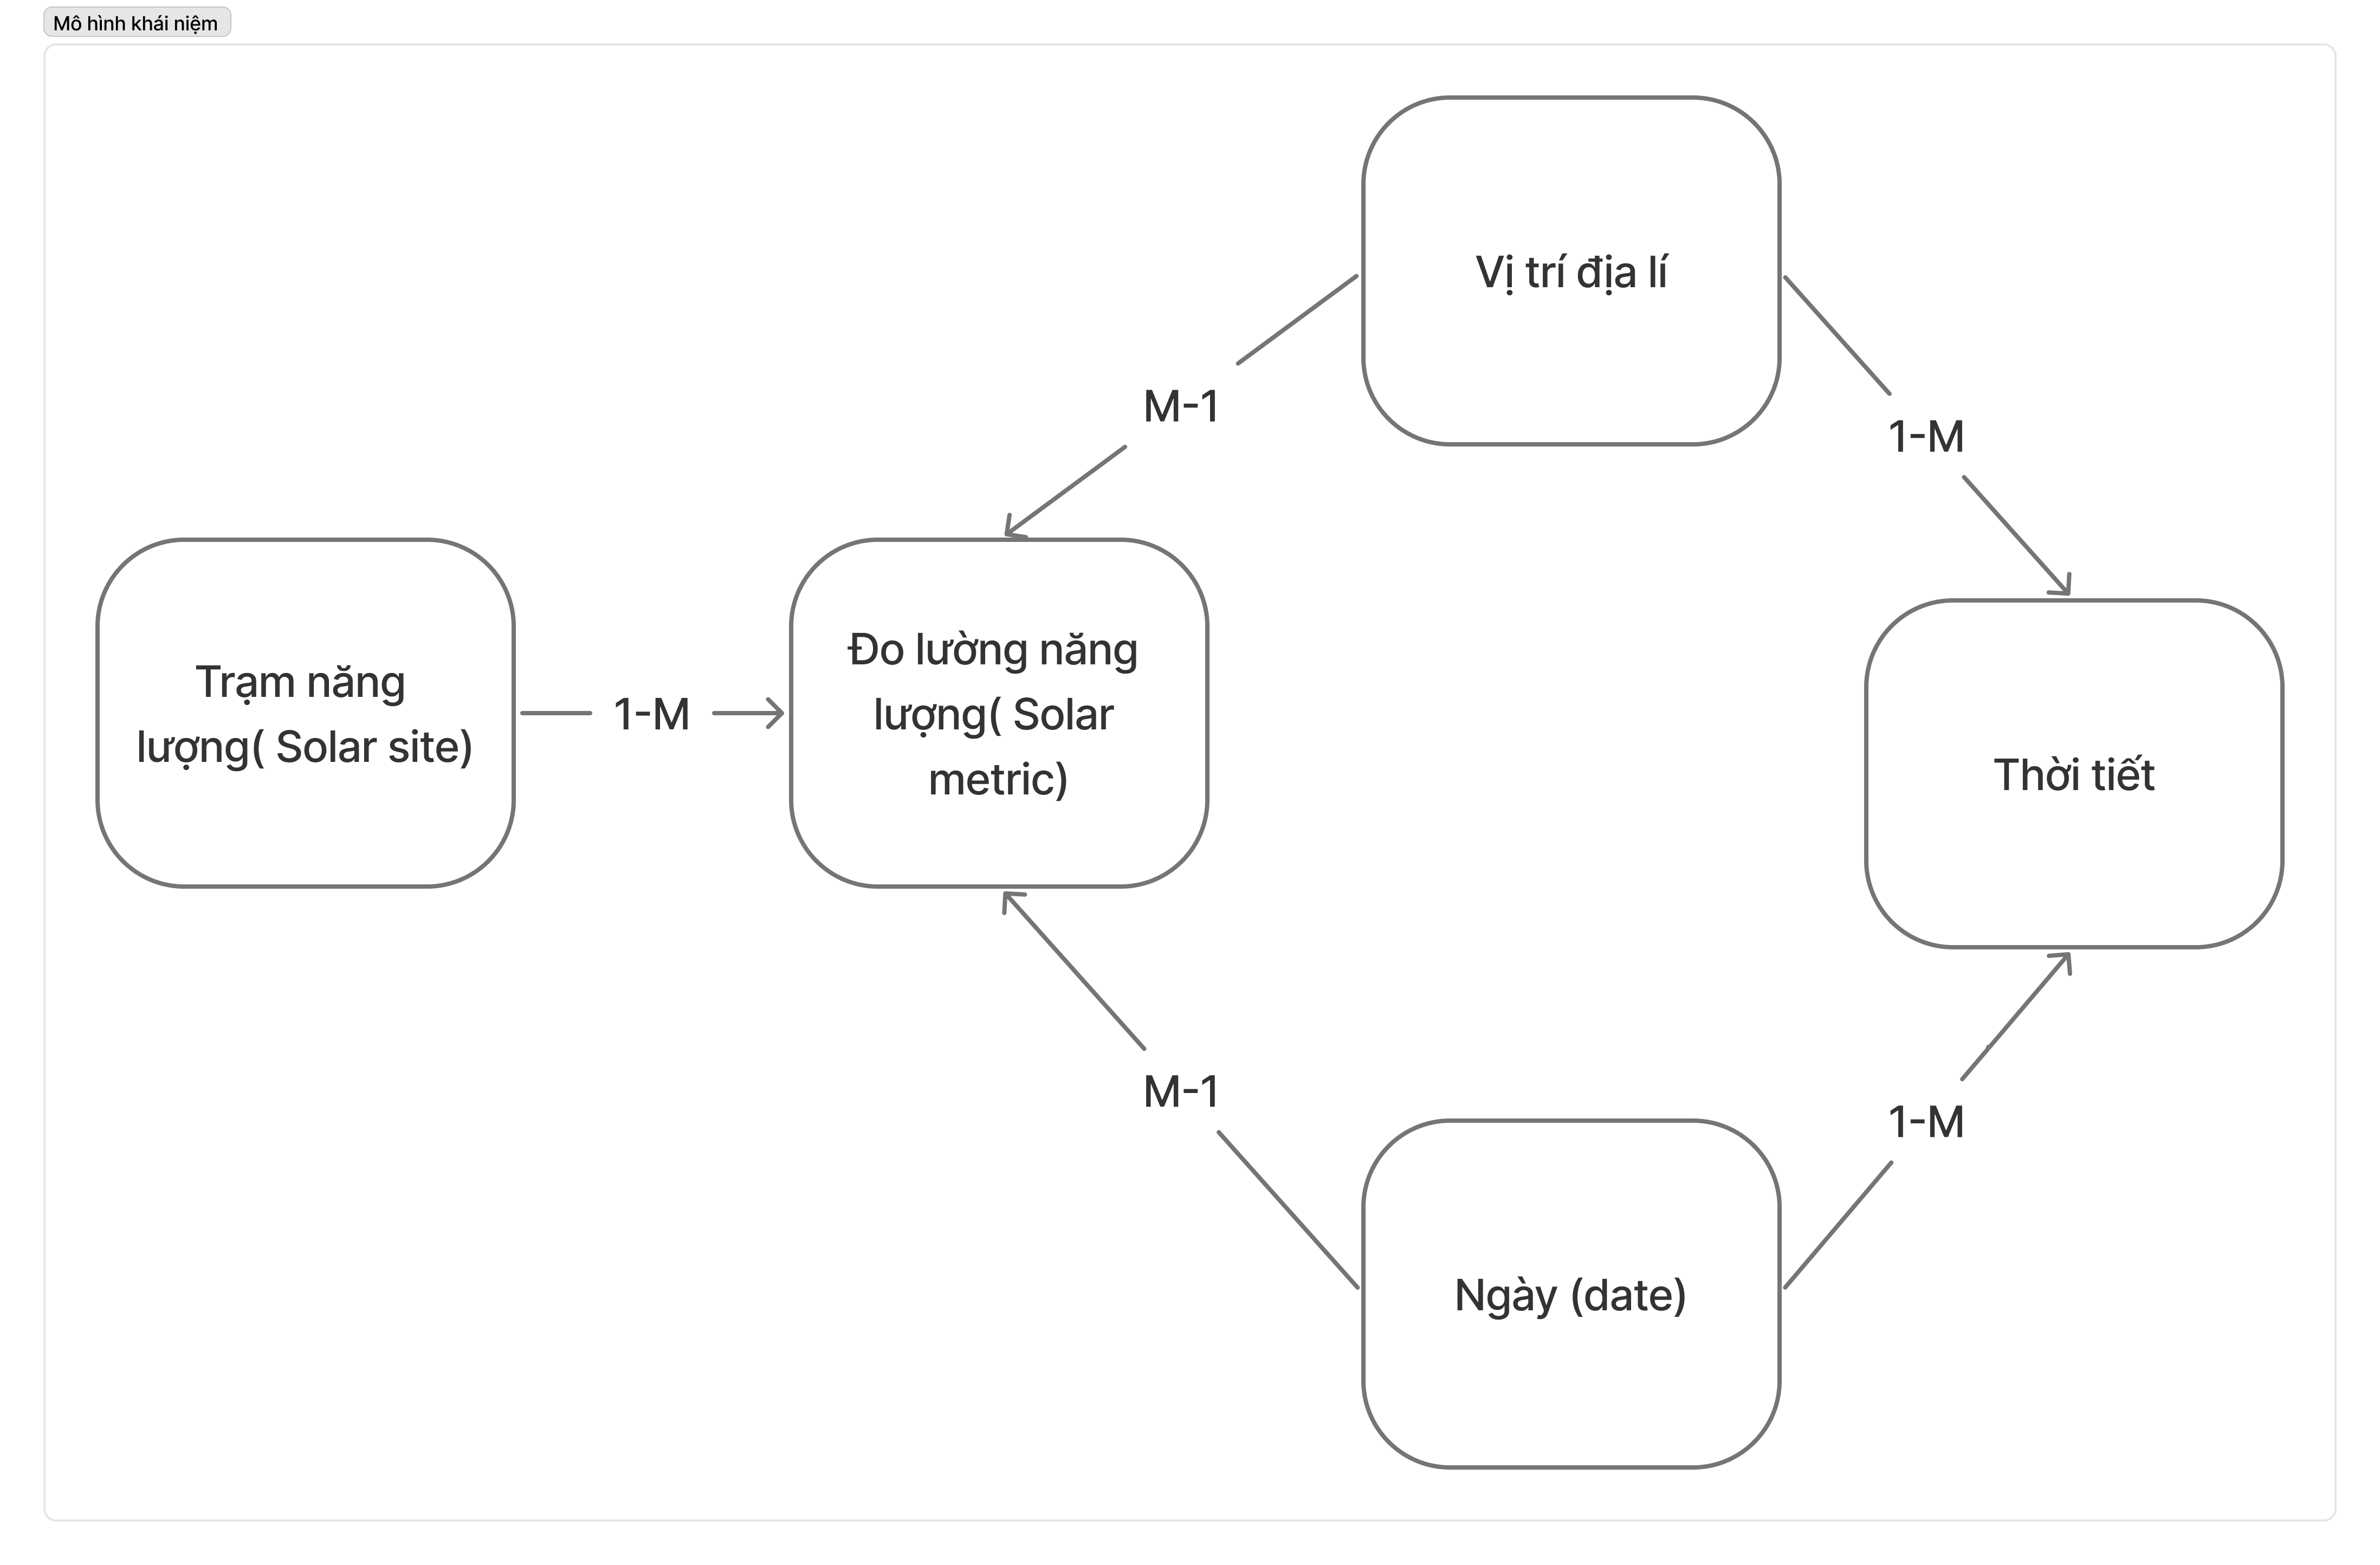
\includegraphics[width=0.88\textwidth]{figures/conceptual_model.png}
\caption{Sơ đồ mô hình khái niệm (Conceptual Model) thể hiện mối quan hệ giữa các thực thể hệ thống điện mặt trời.}
\label{fig:conceptual_model}
\end{figure}

\begin{figure}[H]
\centering
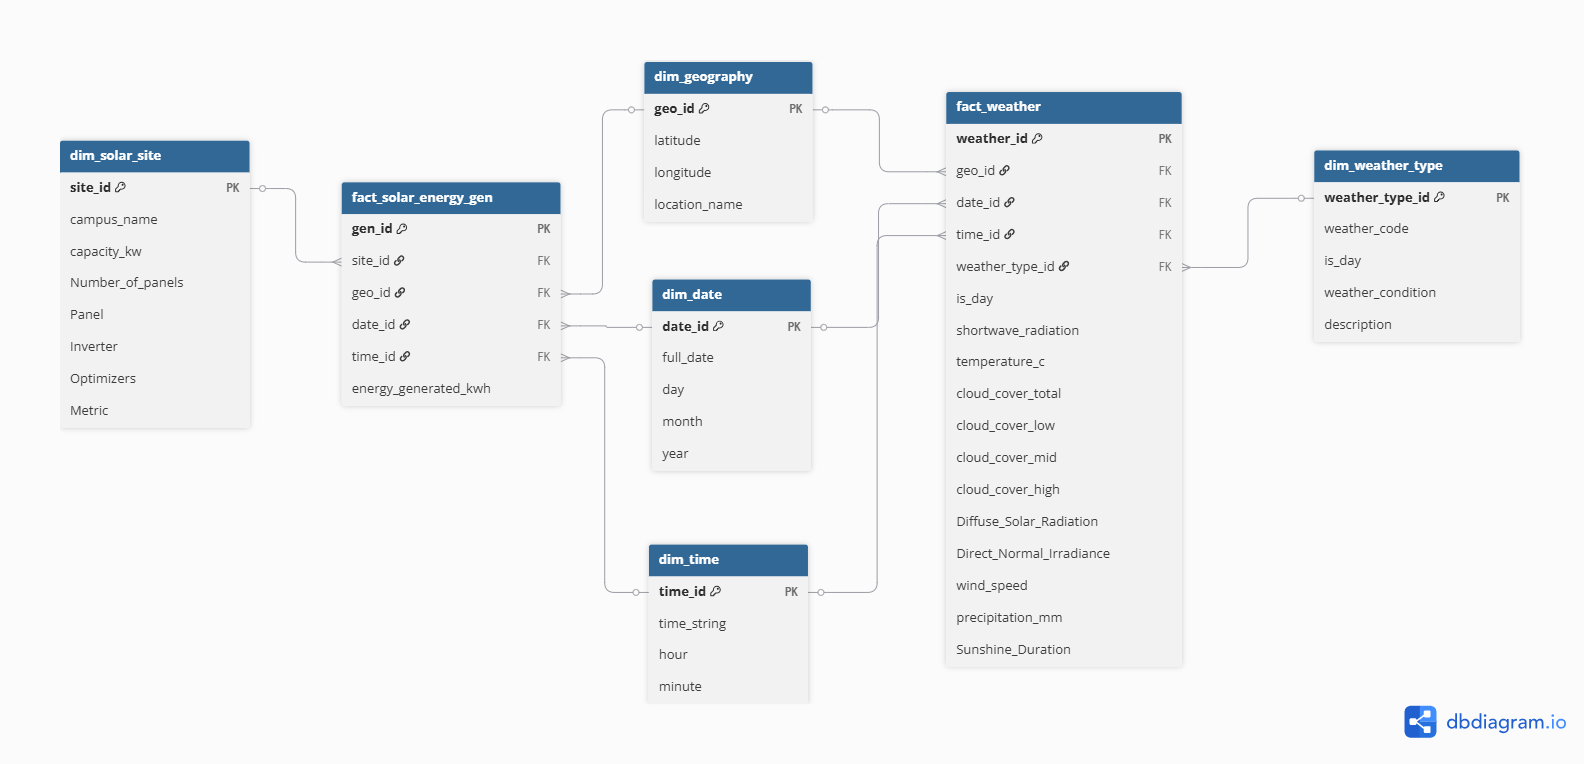
\includegraphics[width=0.92\textwidth]{figures/logical_model.png}
\caption{Sơ đồ mô hình logic (Logical Model) theo kiến trúc Galaxy Schema kết nối 2 bảng Fact và 4 bảng Dimension dùng chung.}
\label{fig:logical_model}
\end{figure}

\begin{figure}[H]
\centering
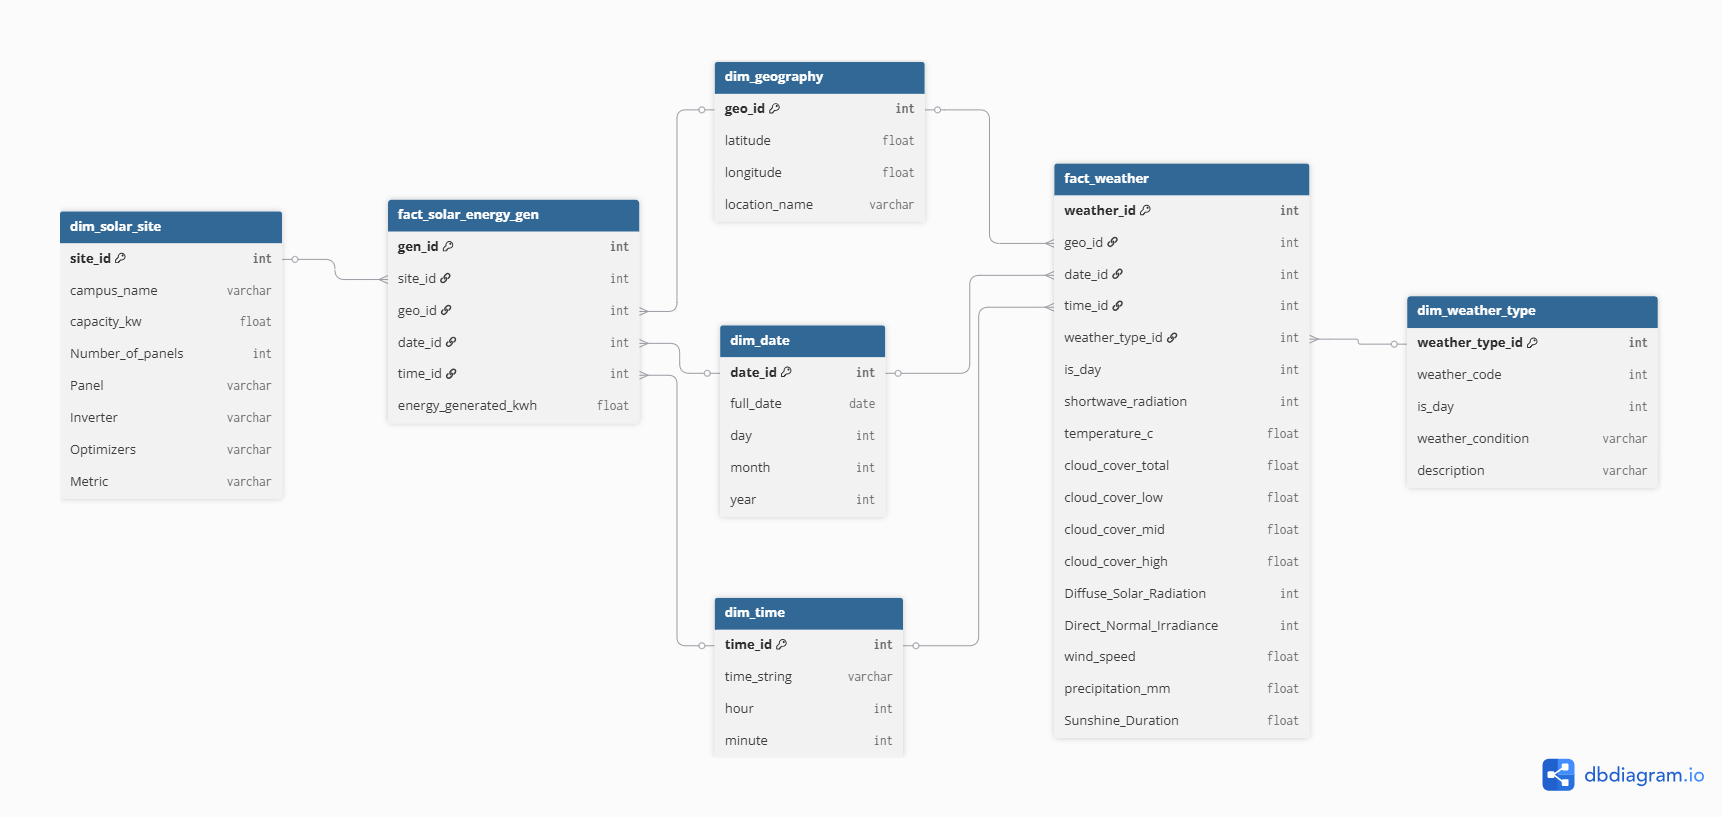
\includegraphics[width=0.95\textwidth]{figures/physical_model.png}
\caption{Sơ đồ mô hình vật lý (Physical Model) triển khai thực tế trên PostgreSQL Supabase.}
\label{fig:physical_model}
\end{figure}

\subsection{Cấu trúc Các Bảng trong Kho Dữ liệu}
\begin{enumerate}[noitemsep]
    \item \textbf{\texttt{dim\_solar\_plant} (Bảng Chiều Trạm phát):} 42 trạm phát với thông tin công suất danh định (\texttt{capacity\_kw}), khuôn viên (\texttt{campus\_name}) và vị trí địa lý.
    \item \textbf{\texttt{dim\_date} (Bảng Chiều Ngày):} 851 ngày lịch biểu trong chu kỳ 28 tháng với các thuộc tính phân tích thời gian.
    \item \textbf{\texttt{dim\_time} (Bảng Chiều Giờ):} 96 mốc thời gian vi mô 15 phút trong ngày.
    \item \textbf{\texttt{dim\_weather\_type} (Bảng Chiều Thời tiết):} Danh mục mã thời tiết chuẩn WMO.
    \item \textbf{\texttt{fact\_solar\_energy\_gen} (Bảng Sự kiện Sản lượng):} $2.731.946$ bản ghi sản lượng 15 phút kèm cờ dị thường và mã lý do.
    \item \textbf{\texttt{fact\_weather} (Bảng Sự kiện Khí tượng):} Các thông số bức xạ và thời tiết chu kỳ 1 giờ.
\end{enumerate}

\section{Tạo Bảng Tổng hợp và Siêu thị Dữ liệu (Siêu thị dữ liệu chuyên đề)}
\label{sec:data_marts}

Để đảm bảo các Dashboard trên Tableau tải tức thời (dưới 1 giây) khi các nhà quản lý thực hiện lọc dữ liệu, module \texttt{aggregate.py} thực hiện tính toán trước (Pre-calculated Aggregation) các bảng Data Marts chuyên biệt:

\begin{itemize}[noitemsep]
    \item \textbf{\texttt{agg\_daily\_plant\_performance.csv}:} Tổng hợp sản lượng hàng ngày, chỉ số PR trung bình, Specific Yield và tổn thất ước tính của 42 trạm phát.
    \item \textbf{\texttt{agg\_monthly\_campus\_summary.csv}:} Tổng hợp sản lượng theo tháng của 4 khuôn viên trường phục vụ báo cáo xu hướng tăng trưởng YoY.
    \item \textbf{\texttt{agg\_hourly\_temperature\_efficiency.csv}:} Ma trận tương quan giữa các dải nhiệt độ, bức xạ và hiệu suất chuyển đổi, làm nổi bật điểm suy giảm hiệu suất do nhiệt độ.
    \item \textbf{\texttt{agg\_anomaly\_diagnostic\_summary.csv}:} Thống kê số lượng và tỷ lệ của 6 mã lý do dị thường theo từng trạm phát phục vụ phân tích bảo trì O\&M.
\end{itemize}

\section{Kiểm tra Tính Toàn vẹn và Bảo mật Dữ liệu}
\label{sec:integrity_security}

\begin{enumerate}[noitemsep]
    \item \textbf{Kiểm tra Khóa ngoại (Anti-Join Check):} Thực hiện truy vấn Anti-Join giữa bảng Fact và Dimension, đảm bảo $100\%$ bản ghi có khóa tham chiếu hợp lệ (0 bản ghi mồ côi).
    \item \textbf{Xác thực Toàn vẹn Dữ liệu (Fingerprint Checksum MD5):} Hàm \texttt{fingerprint\_supabase()} đối chiếu mã băm MD5, tổng sản lượng ($74.982.150{,}45\,\text{kWh}$) và tổng số $2.731.946$ dòng dữ liệu trước và sau quá trình nạp để ngăn ngừa mất mát dữ liệu.
    \item \textbf{Bảo mật Phân quyền (Row-Level Security -- RLS):} Phân quyền truy cập an toàn trên Supabase Cloud, cấp quyền chỉ đọc (Read-only) cho Dashboard Tableau và tài khoản quản trị cho kỹ sư dữ liệu.
\end{enumerate}

\begin{thebibliography}{99}
\addcontentsline{toc}{chapter}{Tài liệu Tham khảo}

\bibitem{wimalaratne2022unisolar}
P.~Wimalaratne, D.~Jayasinghe, và C.~Arachchige,
\newblock ``UNISOLAR: A Comprehensive High-Resolution Open Dataset of 42 Rooftop Photovoltaic Sites,''
\newblock \textit{Data in Brief}, vol.~42, p.~108152, 2022.

\bibitem{openmeteo2023}
Open-Meteo,
\newblock ``Historical Weather API \& ERA5/ERA5-Land Reanalysis Climate Dataset,''
\newblock \textit{Open-Meteo Documentation}, 2023. [Online]. Available: \url{https://open-meteo.com/}.

\bibitem{iea2023pvps}
IEA-PVPS Task 13,
\newblock ``Performance, Operation and Reliability of Photovoltaic Systems: Review of Failures and Degradation Mechanisms,''
\newblock \textit{International Energy Agency Technical Report}, IEA-PVPS T13-15:2023, 2023.

\bibitem{li2025gmmif}
Y.~Li, H.~Zhang, X.~Wang, và J.~Liu,
\newblock ``A Two-Stage Hybrid Outlier Cleaning Framework for Distributed Rooftop Photovoltaic Generation Data Using GMM and Isolation Forest,''
\newblock \textit{IEEE Access}, vol.~13, pp.~24510--24523, 2025.

\bibitem{liu2008isolation}
F.~T.~Liu, K.~M.~Ting, và Z.-H.~Zhou,
\newblock ``Isolation Forest,''
\newblock trong \textit{Proceedings of the IEEE International Conference on Data Mining (ICDM)}, 2008, pp.~413--422.

\bibitem{bishop2006pattern}
C.~M.~Bishop,
\newblock \textit{Pattern Recognition and Machine Learning},
\newblock Springer, New York, 2006.

\bibitem{tukey1977eda}
J.~W.~Tukey,
\newblock \textit{Exploratory Data Analysis},
\newblock Addison-Wesley, Reading, MA, 1977.

\bibitem{chandola2009anomaly}
V.~Chandola, A.~Banerjee, và V.~Kumar,
\newblock ``Anomaly Detection: A Survey,''
\newblock \textit{ACM Computing Surveys}, vol.~41, no.~3, pp.~1--58, 2009.

\bibitem{kim2019missing}
G.~Kim, S.~Park, và S.~Lee,
\newblock ``Physical Constraint Imputation and Spatial Interpolation for Missing Solar Irradiance Data,''
\newblock \textit{Solar Energy}, vol.~188, pp.~754--765, 2019.

\bibitem{roy2025hourly}
A.~Roy, M.~Rahman, và K.~Chowdhury,
\newblock ``Hourly-Binned Regressors Outperform Complex Deep Learning for Local Solar Generation Forecasting,''
\newblock \textit{Applied Energy}, vol.~355, p.~122301, 2025.

\bibitem{haurwitz1945}
B.~Haurwitz,
\newblock ``Insolation in Relation to Cloudiness and Cloud Density,''
\newblock \textit{Journal of Meteorology}, vol.~2, no.~3, pp.~154--166, 1945.

\bibitem{bailey2024}
J.~Bailey, R.~Miller, và S.~Thompson,
\newblock ``Clear-Sky PV Generation Modeling Under Complex Atmospheric Conditions,''
\newblock \textit{Renewable Energy}, vol.~219, pp.~119--131, 2024.

\bibitem{engerer2014kpv}
N.~A.~Engerer và F.~P.~Mills,
\newblock ``Validating the PV Clear-Sky Index and Modeling Rooftop Solar Production,''
\newblock \textit{Solar Energy}, vol.~105, pp.~619--632, 2014.

\bibitem{dev2018tes}
S.~Dev, F.~M.~Savoy, Y.~H.~Lee, và S.~Winkler,
\newblock ``High-Resolution Weather and Irradiance Monitoring for PV Plant Management,''
\newblock \textit{IEEE Transactions on Geoscience and Remote Sensing}, vol.~56, no.~4, pp.~2120--2132, 2018.

\bibitem{pin2025wape}
E.~Pin, M.~Rossi, và T.~Nguyen,
\newblock ``Weighted Absolute Percentage Error (WAPE) as a Robust Standard for Intermittent Renewable Energy Forecasting Metrics,''
\newblock \textit{Energy Reports}, vol.~11, pp.~402--415, 2025.

\bibitem{lundberg2017shap}
S.~M.~Lundberg và S.-I.~Lee,
\newblock ``A Unified Approach to Interpreting Model Predictions,''
\newblock trong \textit{Advances in Neural Information Processing Systems (NeurIPS)}, vol.~30, 2017, pp.~4765--4774.

\bibitem{zhang2013metrics}
J.~Zhang, B.-M.~Hodge, và A.~Florita,
\newblock ``Comprehensive Evaluation of Solar Irradiance and Power Forecasting Metrics,''
\newblock \textit{Journal of Renewable and Sustainable Energy}, vol.~5, no.~4, p.~043126, 2013.

\bibitem{lonij2012tucson}
V.~P.~Lonij, A.~E.~Brooks, A.~D.~Cronin, và F.~J.~Rocha,
\newblock ``Intra-Hour Solar Forecasting with High-Density PV Networks and Cloud Tracking,''
\newblock \textit{Solar Energy}, vol.~86, no.~5, pp.~1450--1461, 2012.

\bibitem{taylor2018prophet}
S.~J.~Taylor và B.~Letham,
\newblock ``Forecasting at Scale,''
\newblock \textit{The American Statistician}, vol.~72, no.~1, pp.~37--45, 2018.

\bibitem{box2015time}
G.~E.~P.~Box, G.~M.~Jenkins, G.~C.~Reinsel, và G.~M.~Ljung,
\newblock \textit{Time Series Analysis: Forecasting and Control}, 5th ed.,
\newblock John Wiley \& Sons, Hoboken, NJ, 2015.

\bibitem{ke2017lightgbm}
G.~Ke, Q.~Meng, T.~Finley, T.~Wang, W.~Chen, W.~Ma, Q.~Ye, và T.-Y.~Liu,
\newblock ``LightGBM: A Highly Efficient Gradient Boosting Decision Tree,''
\newblock trong \textit{Advances in Neural Information Processing Systems (NeurIPS)}, vol.~30, 2017, pp.~3146--3154.

\bibitem{chen2016xgboost}
T.~Chen và C.~Guestrin,
\newblock ``XGBoost: A Scalable Tree Boosting System,''
\newblock trong \textit{Proceedings of the ACM SIGKDD International Conference on Knowledge Discovery and Data Mining}, 2016, pp.~785--794.

\bibitem{kimball2013dwh}
R.~Kimball và M.~Ross,
\newblock \textit{The Data Warehouse Toolkit: The Definitive Guide to Dimensional Modeling}, 3rd ed.,
\newblock John Wiley \& Sons, Indianapolis, IN, 2013.

\bibitem{wmo2021guide}
World Meteorological Organization (WMO),
\newblock \textit{Guide to Instruments and Methods of Observation: Volume I -- Measurement of Meteorological Variables},
\newblock WMO-No. 8, Geneva, Switzerland, 2021.

\bibitem{supabase2024}
Supabase Inc.,
\newblock ``PostgreSQL Database \& Row-Level Security for Modern Analytics Architecture,''
\newblock \textit{Supabase Technical Architecture Documentation}, 2024. [Online]. Available: \url{https://supabase.com/docs}.

\bibitem{pedregosa2011sklearn}
F.~Pedregosa et~al.,
\newblock ``Scikit-learn: Machine Learning in Python,''
\newblock \textit{Journal of Machine Learning Research}, vol.~12, pp.~2825--2830, 2011.

\bibitem{tableau2023guidelines}
Tableau Software (Salesforce),
\newblock \textit{Visual Analysis Best Practices: A Guide to Creating Meaningful Dashboards},
\newblock Seattle, WA, 2023.

\end{thebibliography}


\end{document}
